%--------------------------------------------------------------------------------------------
% Plotting model output
%--------------------------------------------------------------------------------------------

\chapter{Visualization}
\label{chap:mpas_visualization}

This chapter discusses visualization tools that may be used by all cores.  For instructions on additional visualization tools for this core, see Chapter \ref{chap:\core_visualization}.

\section{ParaView}

ParaView may be used to visualize MPAS initialization, output, and restart files.  It includes a reader that was specifically designed to read MPAS NetCDF files, including Cartesian and spherical domains.  At this time, only cell-centered quantities may be plotted with ParaView.  Variables located at edges and vertices must be interpolated to cell centers for visualization.

ParaView is freely available for download at \url{http://www.paraview.org}.  Binary installations are available for Windows, Mac, and Linux, as well as source code files and tutorials.  From the ParaView website:
\begin{quotation}
ParaView is an open-source, multi-platform data analysis and visualization application. ParaView users can quickly build visualizations to analyze their data using qualitative and quantitative techniques. The data exploration can be done interactively in 3D or programmatically using ParaView's batch processing capabilities.  ParaView was developed to analyze extremely large datasets using distributed memory computing resources. It can be run on supercomputers to analyze datasets of terascale as well as on laptops for smaller data.
\end{quotation}

To visualize an MPAS cell-centered variable in ParaView, open the file and choose {\tt MPAS NetCDF (Unstructured)} as the file format.  In the lower left Object Inspector panel, choose your variables of interest (Figure \ref{fig:ParaviewExample}).  For large data sets, loading fewer variables will result in less wait time.  Options are available for latitude-longitude projections, vertical level, etc.  Click the 'Apply' button to load the data set.  In the toolbars at the top, choose the variable to plot from the pull-down menu, and 'Surface' for the type of visualization.  The color bar button displays a color bar, and the color scale editor button allows the user to manually change the color bar type and extents.  The Filters menu provides computational tools for interactive data manipulation.  Movies, in avi format or as individual frames, may be conveniently created with the {\tt Save Animation} tool in the File menu.

\begin{figure}[htb]
\begin{center}
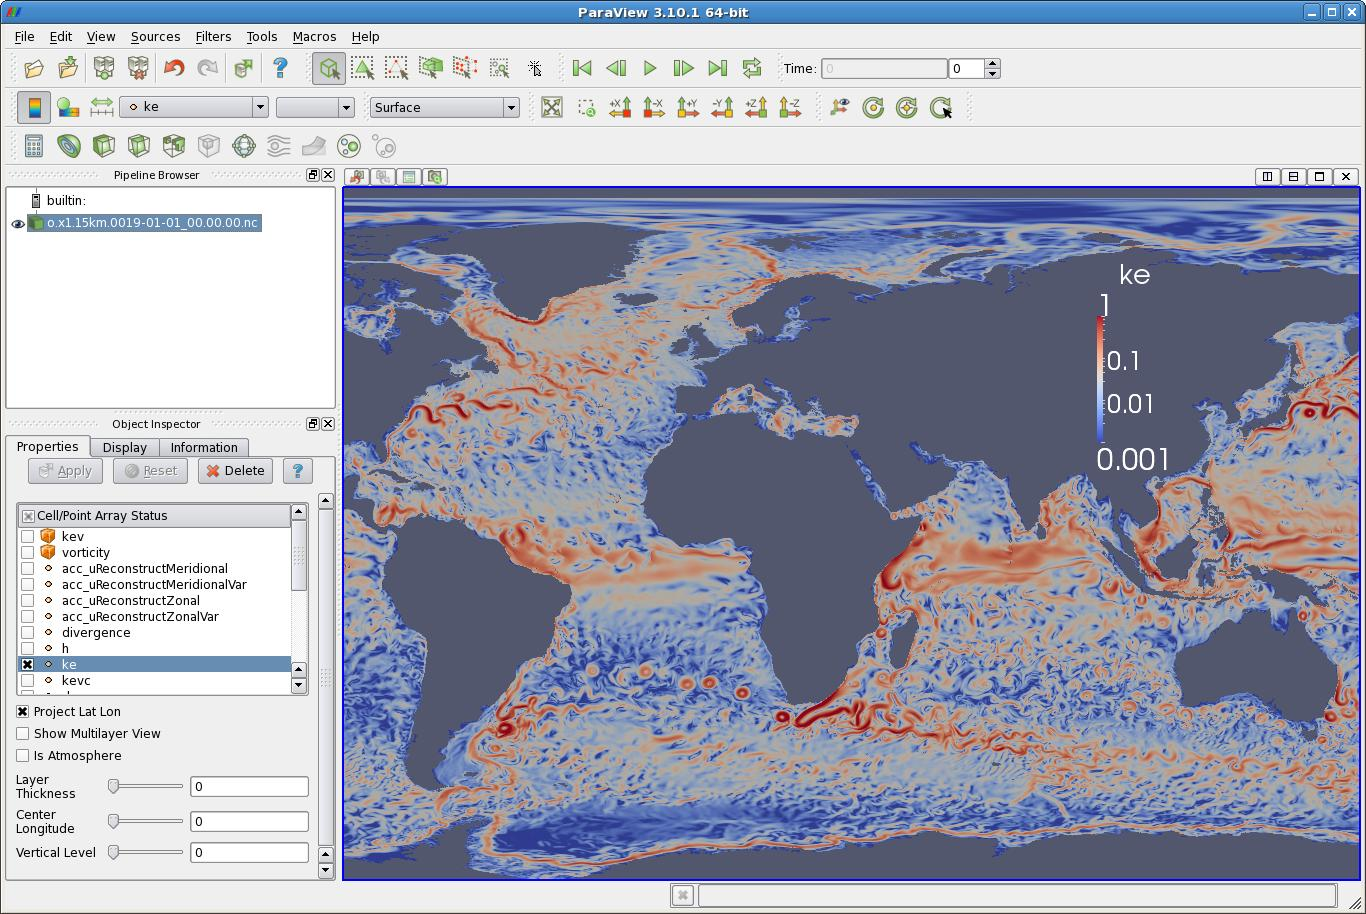
\includegraphics[width=6.5in]{shared/figures/ParaviewExample.jpg}
\caption{Example of ParaView to view an MPAS NetCDF file.}
\label{fig:ParaviewExample}
\end{center}
\end{figure}

Paraview may be used to view the grid from any MPAS NetCDF file by choosing {\tt Wireframe} or {\tt Suface With Edges} from the visualization-type pull-down menu (Figure \ref{fig:ParaviewExampleEdges}).  This produces a view of the Delaunay triangulation, which is the dual mesh to the primal Voronoi cell grid (Figure \ref{figure:variablePosition}).  Paraview plots all variables by interpolating colors between each corner of the Delaunay triangles.  These corners are the cell-center locations of the primal grid.

\begin{figure}[htb]
\begin{center}
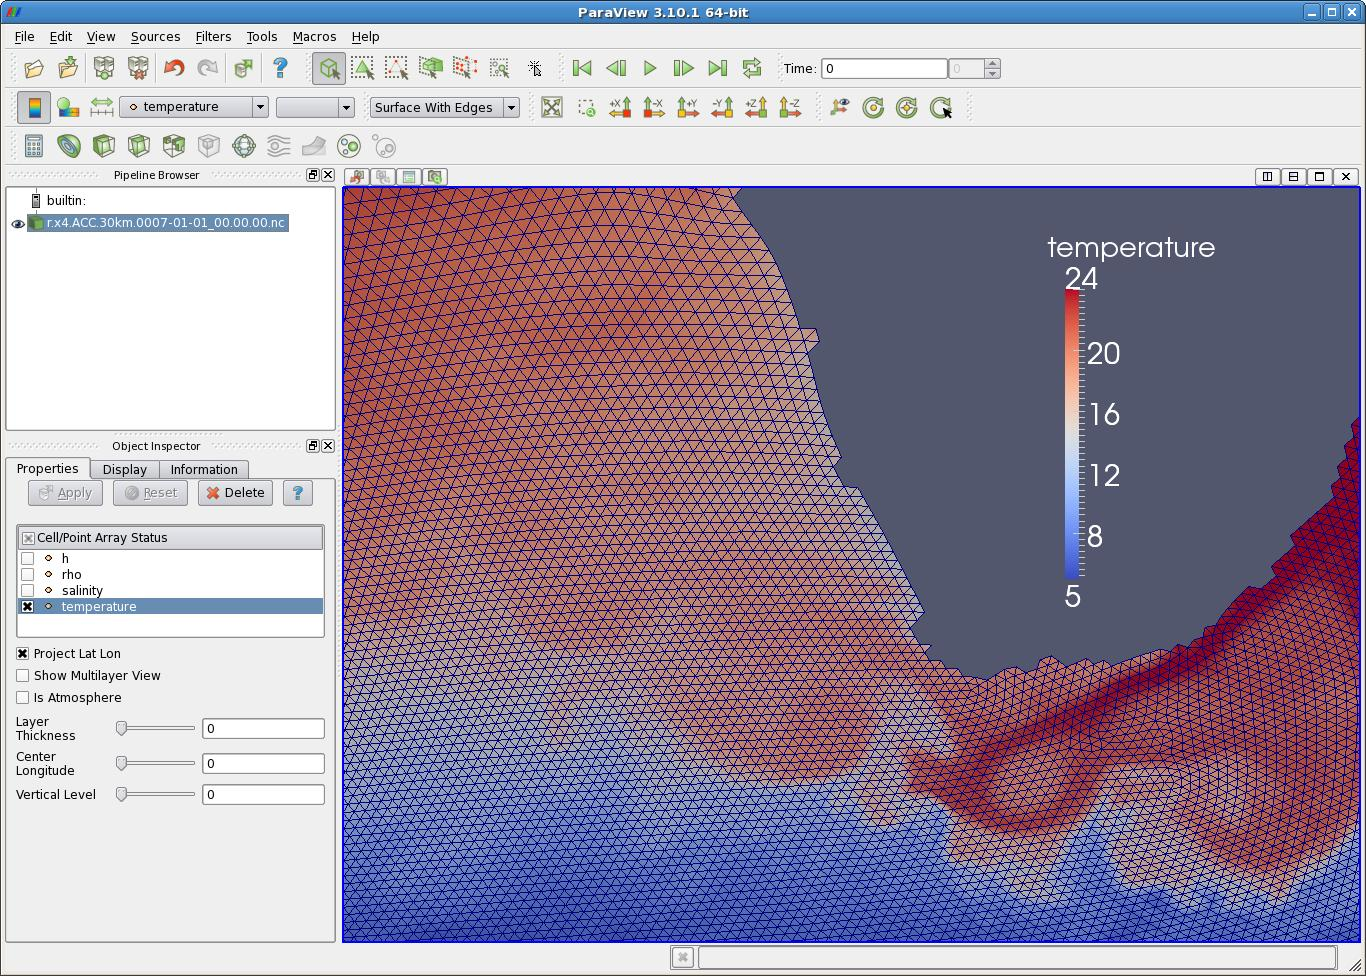
\includegraphics[width=6.5in]{shared/figures/ParaviewExampleEdges.jpg}
\caption{Example of visualizing the dual mesh from an MPAS NetCDF file.}
\label{fig:ParaviewExampleEdges}
\end{center}
\end{figure}

